% Document/LinearAlgebra/VectorSpaces/LinearMaps/Definition.tex
% Section: Definition of Linear Maps

\newpage
\section{Linear Transformations}

\begin{intuition}[The Category $K$-Vect]
    Having defined vector spaces as the objects of study, we now define the \textbf{morphisms}
    between them. In category-theoretic terms, a $K$-vector space homomorphism is a function
    that preserves the vector space structure. The collection of all such morphisms from $U$ to $V$
    is denoted
    \[
        \Hom[K]{U}{V} = \Set{T : U \to V \mid T \text{ is $K$-linear}}
    \]
    Together with composition of morphisms, this forms the \textbf{category $K$-Vect} of
    $K$-vector spaces and $K$-linear maps.
\end{intuition}

\begin{definition}[Linear Transformation]\label{def:linear-map}
    Let $U$ and $V$ be $K$-vector spaces. A function $T: U \to V$ is a \textbf{linear transformation}
    (or \textbf{linear map}, or \textbf{$K$-linear map}) if it preserves the vector space structure:
    \begin{enumerate}
        \item $\Forall :{u, v \in U}{T(u + v) = T(u) + T(v)}$ (additivity)
        \item $\Forall :{a \in K}{\Forall :{u \in U}{T(au) = aT(u)}}$ (homogeneity)
    \end{enumerate}
    Equivalently, $T$ is linear iff 
    $\Forall :{a, b \in K}{\Forall :{u, v \in U}{T(au + bv) = aT(u) + bT(v)}}$.
\end{definition}

\begin{proposition}[Composition of Linear Maps]\label{prop:composition-linear}
    If $T: U \to V$ and $S: V \to W$ are linear, then $\Composition{S}{T}: U \to W$ is linear.
\end{proposition}

\begin{proof}
    For any $a, b \in K$ and $u_1, u_2 \in U$:
    \begin{align*}
        (\Composition{S}{T})(au_1 + bu_2) &= S(T(au_1 + bu_2)) \\
        &= S(aT(u_1) + bT(u_2)) \\
        &= aS(T(u_1)) + bS(T(u_2)) \\
        &= a(\Composition{S}{T})(u_1) + b(\Composition{S}{T})(u_2)
    \end{align*}
\end{proof}

\begin{remark}[Category Structure]
    The composition of linear maps is associative (inherited from function composition),
    and $\Identity{V}$ serves as the identity morphism. Thus $K$-Vect forms a category.
\end{remark}

\begin{proposition}[Basic Properties of Linear Maps]\label{prop:linear-map-basic}
    Let $T: U \to V$ be a linear map. Then:
    \begin{enumerate}
        \item $T(0_U) = 0_V$
        \item $T(-u) = -T(u)$ for all $u \in U$
        \item $T\left(\sum_{i \in n} a_i u_i\right) = \sum_{i \in n} a_i T(u_i)$ for any finite linear combination
    \end{enumerate}
\end{proposition}

\begin{proof}
    \textbf{(1)}: $T(0_U) = T(0 \cdot 0_U) = 0 \cdot T(0_U) = 0_V$.
    
    \textbf{(2)}: $T(-u) = T((-1) \cdot u) = (-1) \cdot T(u) = -T(u)$.
    
    \textbf{(3)}: By induction on $n$ using additivity and homogeneity.
\end{proof}

\begin{example}[Basic Linear Maps]\label{ex:basic-linear-maps}
    Consider the following examples of linear maps:
    \begin{enumerate}
        \item \textbf{Scalar multiplication}: For any $a \in K$, the map $T: V \to V$ defined by
              $T(v) = av$ is linear (verify: $T(bu + cv) = a(bu + cv) = abu + acv = bT(u) + cT(v)$).
        \item \textbf{Identity}: The map $\Identity{V}: V \to V$ with $\Identity{V}(v) = v$ is linear.
        \item \textbf{Zero map}: The map $0: U \to V$ with $0(u) = 0_V$ for all $u \in U$ is linear.
        \item \textbf{Inclusion}: If $W \Subspace[K] V$, the inclusion $\iota: W \hookrightarrow V$ is linear.
        \item \textbf{Derivative}: The map $D: K[X] \to K[X]$ with $D(p) = p'$ (formal derivative) is linear.
        \item \textbf{Evaluation}: For fixed $a \in K$, the map $\text{ev}_a: K[X] \to K$ with 
              $\text{ev}_a(p) = p(a)$ is linear.
        \item \textbf{Coordinate projection}: For any index set $I$ and $i \in I$:
              \begin{itemize}
                  \item $\pi_i: K^I \to K$ with $\pi_i(f) = f(i)$ is linear
                  \item $\pi_i: K^{(I)} \to K$ with $\pi_i(f) = f(i)$ is linear (restriction to finite support)
              \end{itemize}
    \end{enumerate}
\end{example}

\begin{figure}[h]
    \centering
    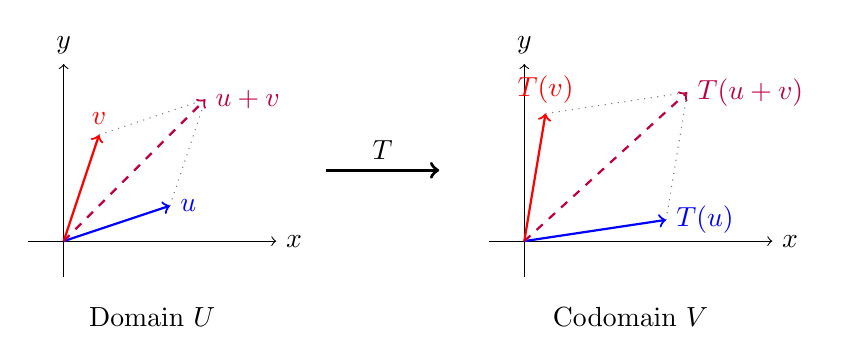
\begin{tikzpicture}[scale=0.9]
        % Domain - R^2
        \begin{scope}
            \draw[->] (-0.5,0) -- (3,0) node[right] {$x$};
            \draw[->] (0,-0.5) -- (0,2.5) node[above] {$y$};
            
            % Vectors u and v
            \draw[->, thick, blue] (0,0) -- (1.5,0.5) node[right] {$u$};
            \draw[->, thick, red] (0,0) -- (0.5,1.5) node[above] {$v$};
            
            % Sum u+v
            \draw[->, thick, purple, dashed] (0,0) -- (2,2) node[right] {$u+v$};
            \draw[dotted, gray] (1.5,0.5) -- (2,2);
            \draw[dotted, gray] (0.5,1.5) -- (2,2);
            
            \node[below] at (1.25,-0.8) {Domain $U$};
        \end{scope}
        
        % Arrow for transformation
        \draw[->, very thick] (3.7,1) -- (5.3,1) node[midway, above] {$T$};
        
        % Codomain - with T preserving addition
        \begin{scope}[xshift=6.5cm]
            \draw[->] (-0.5,0) -- (3.5,0) node[right] {$x$};
            \draw[->] (0,-0.5) -- (0,2.5) node[above] {$y$};
            
            % T(u) and T(v)
            \draw[->, thick, blue] (0,0) -- (2,0.3) node[right] {$T(u)$};
            \draw[->, thick, red] (0,0) -- (0.3,1.8) node[above] {$T(v)$};
            
            % T(u+v) = T(u) + T(v)
            \draw[->, thick, purple, dashed] (0,0) -- (2.3,2.1) node[right] {$T(u+v)$};
            \draw[dotted, gray] (2,0.3) -- (2.3,2.1);
            \draw[dotted, gray] (0.3,1.8) -- (2.3,2.1);
            
            \node[below] at (1.5,-0.8) {Codomain $V$};
        \end{scope}
    \end{tikzpicture}
    \caption{A linear map $T$ preserves vector addition: the parallelogram law holds in both domain and codomain,
    ensuring $T(u + v) = T(u) + T(v)$.}
    \label{fig:linear-map-additivity}
\end{figure}

\begin{example}[Non-Linear Maps]\label{ex:non-linear}
    The following maps are \textbf{not} linear:
    \begin{enumerate}
        \item \textbf{Translation}: $T(v) = v + c$ for nonzero $c$ (fails $T(0) = 0$).
        \item \textbf{Squaring}: $T: \bb{R} \to \bb{R}$ with $T(x) = x^2$ (fails homogeneity: $T(2x) = 4x^2 \neq 2x^2$).
        \item \textbf{Norm}: $T: \bb{R}^n \to \bb{R}$ with $T(v) = \|v\|$ (fails additivity in general).
    \end{enumerate}
\end{example}

\newpage
\section{Universal Property of Vector Spaces}

\begin{theorem}[Universal Property of Vector Spaces (Free Object)]%
    \label{thm:vector-space-universal}
    Let $V$ be a $K$-vector space with basis $B$, let $W$ be any $K$-vector space, and let
    $f: B \to W$ be any function. Then there exists a \textbf{unique} linear map $T: V \to W$
    such that $\Restriction{T}[B] = f$.
    
    \begin{center}
    \begin{tikzcd}
        B \arrow[r, hook, "\iota"] \arrow[dr, "f"'] & V \arrow[d, dashed, "\exists! T"] \\
        & W
    \end{tikzcd}
    \end{center}
    
    This characterizes vector spaces with bases as \textbf{free objects} in $K$-Vect:
    the vector space $V$ is ``freely generated'' by the set $B$.
\end{theorem}

\begin{proof}
    \textbf{Existence}: Every $v \in V$ has a unique representation $v = \sum_{b \in F} a_b b$ for
    some finite $F \subseteq B$ with nonzero coefficients $a_b$. Define
    \[
        T(v) = \sum_{b \in F} a_b f(b)
    \]
    
    We verify $T$ is linear. Let $v = \sum_{b} a_b b$ and $w = \sum_{b} c_b b$ (with zero coefficients
    for $b$ not in the support). For $\alpha, \beta \in K$:
    \begin{align*}
        T(\alpha v + \beta w) &= T\left(\sum_{b} (\alpha a_b + \beta c_b) b\right) \\
        &= \sum_{b} (\alpha a_b + \beta c_b) f(b) \\
        &= \alpha \sum_{b} a_b f(b) + \beta \sum_{b} c_b f(b) \\
        &= \alpha T(v) + \beta T(w)
    \end{align*}
    
    By construction, $T(b) = 1 \cdot f(b) = f(b)$ for all $b \in B$, so $\Restriction{T}[B] = f$.
    
    \textbf{Uniqueness}: Let $S: V \to W$ be linear with $\Restriction{S}[B] = f$. For any 
    $v = \sum_{b \in F} a_b b$:
    \[
        S(v) = S\left(\sum_{b \in F} a_b b\right) = \sum_{b \in F} a_b S(b) = \sum_{b \in F} a_b f(b) = T(v)
    \]
    Thus $S = T$.
\end{proof}

\begin{figure}[h]
    \centering
    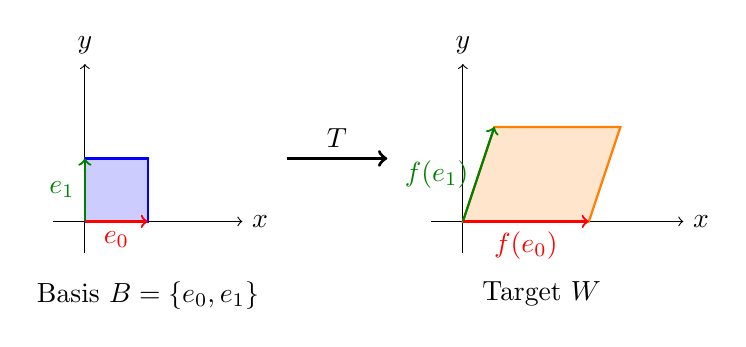
\begin{tikzpicture}[scale=0.8]
        % Original unit square
        \begin{scope}
            \draw[->] (-0.5,0) -- (2.5,0) node[right] {$x$};
            \draw[->] (0,-0.5) -- (0,2.5) node[above] {$y$};
            \fill[blue!20] (0,0) -- (1,0) -- (1,1) -- (0,1) -- cycle;
            \draw[blue, thick] (0,0) -- (1,0) -- (1,1) -- (0,1) -- cycle;
            \draw[->, thick, red] (0,0) -- (1,0) node[midway, below] {$e_0$};
            \draw[->, thick, green!50!black] (0,0) -- (0,1) node[midway, left] {$e_1$};
            \node[below] at (1,-0.8) {Basis $B = \{e_0, e_1\}$};
        \end{scope}
        
        % Arrow for transformation
        \draw[->, very thick] (3.2,1) -- (4.8,1) node[midway, above] {$T$};
        
        % Transformed parallelogram
        \begin{scope}[xshift=6cm]
            \draw[->] (-0.5,0) -- (3.5,0) node[right] {$x$};
            \draw[->] (0,-0.5) -- (0,2.5) node[above] {$y$};
            \fill[orange!20] (0,0) -- (2,0) -- (2.5,1.5) -- (0.5,1.5) -- cycle;
            \draw[orange, thick] (0,0) -- (2,0) -- (2.5,1.5) -- (0.5,1.5) -- cycle;
            \draw[->, thick, red] (0,0) -- (2,0) node[midway, below] {$f(e_0)$};
            \draw[->, thick, green!50!black] (0,0) -- (0.5,1.5) node[midway, left] {$f(e_1)$};
            \node[below] at (1.25,-0.8) {Target $W$};
        \end{scope}
    \end{tikzpicture}
    \caption{The universal property in action: specifying $f(e_0)$ and $f(e_1)$ uniquely determines the linear map $T$.
    The unit square spanned by $\{e_0, e_1\}$ maps to the parallelogram spanned by $\{f(e_0), f(e_1)\}$.}
    \label{fig:universal-property}
\end{figure}
\begin{theorem}[Equivalent Characterizations of Free Vector Spaces]%
    \label{thm:free-vector-space-equiv}
    For a $K$-vector space $V$, the following are equivalent:
    \begin{enumerate}
        \item $V$ has a basis
        \item $V$ satisfies the universal property: for some set $B \subseteq V$ and any $f: B \to W$,
              there exists a unique linear extension $T: V \to W$
        \item $V$ is an internal direct sum of one-dimensional subspaces:
              $V = \DirectSum{i \in I}{\Span[K]{\{v_i\}}}$ for some family of nonzero vectors $(v_i)_{i \in I}$
    \end{enumerate}
\end{theorem}

\begin{proof}
    \textbf{(1) $\Rightarrow$ (2)}: This is exactly the content of Theorem~\ref{thm:vector-space-universal}.
    
    \textbf{(2) $\Rightarrow$ (1)}: We show the set $B$ satisfying the universal property must be a basis.
    
    \textit{Linear independence}: Suppose $\sum_{b \in F} a_b b = 0$ for some finite $F \subseteq B$
    with not all $a_b = 0$. Pick $b_0 \in F$ with $a_{b_0} \neq 0$.
    Consider two maps from $B$ to $K$:
    \begin{itemize}
        \item $f_1: B \to K$ defined by $f_1(b) = 0$ for all $b \in B$
        \item $f_2: B \to K$ defined by $f_2(b_0) = 1$ and $f_2(b) = 0$ for $b \neq b_0$
    \end{itemize}
    Let $T_1, T_2: V \to K$ be the unique linear extensions. Then:
    \[
        T_1\left(\sum_{b \in F} a_b b\right) = \sum_{b \in F} a_b f_1(b) = 0
    \]
    \[
        T_2\left(\sum_{b \in F} a_b b\right) = \sum_{b \in F} a_b f_2(b) = a_{b_0} \neq 0
    \]
    But $\sum a_b b = 0$, so $T_1(0) = 0 = T_2(0)$, contradiction. Thus $B$ is linearly independent.
    
    \textit{Generation}: Consider the identity map $\Identity{V}: V \to V$.
    The inclusion $\iota: B \hookrightarrow V$ extends to some linear $T: V \to V$ with $T|_B = \iota$.
    But $\Identity{V}$ also satisfies $\Identity{V}|_B = \iota$.
    By uniqueness, $T = \Identity{V}$.
    Since $T$ is determined by its values on $B$, every $v \in V$ is a linear combination of elements of $B$.
    Thus $B$ generates $V$.
    
    \textbf{(1) $\Leftrightarrow$ (3)}: If $B = \{b_i\}_{i \in I}$ is a basis, then 
    $V = \DirectSum{i \in I}{\Span[K]{\{b_i\}}}$ (internal direct sum decomposition).
    Conversely, if $V = \DirectSum{i \in I}{\Span[K]{\{v_i\}}}$ with each $v_i \neq 0$,
    then $\{v_i\}_{i \in I}$ is a basis.
\end{proof}

\begin{corollary}[Every Vector Space is Free]\label{cor:every-vs-free}
    Every $K$-vector space is free, since every vector space has a basis (by Zorn's lemma).
\end{corollary}

\begin{corollary}[Linear Maps Determined by Basis Values]\label{cor:linear-map-basis}
    A linear map $T: V \to W$ is uniquely determined by its values on any basis of $V$.
    In particular, for finite-dimensional spaces, every linear map $T: K^n \to K^m$ is uniquely 
    determined by the images of the standard basis vectors $T(e_0), \ldots, T(e_{n-1}) \in K^m$.
\end{corollary}

\begin{proposition}[Images and Preimages of Subspaces]\label{prop:image-preimage-subspace}
    Let $T: U \to V$ be a linear map.
    \begin{enumerate}
        \item If $W \Subspace[K] U$, then $\DirectImage{T}{W} \Subspace[K] V$.
        \item If $W \Subspace[K] V$, then $\InverseImage{T}{W} \Subspace[K] U$.
    \end{enumerate}
\end{proposition}

\begin{proof}
    \textbf{(1)}: We verify the subspace criterion.
    \begin{itemize}
        \item $\DirectImage{T}{W} \neq \emptyset$: Since $0_U \in W$, we have $T(0_U) = 0_V \in \DirectImage{T}{W}$.
        \item Closure: Let $v_1, v_2 \in \DirectImage{T}{W}$, so $v_i = T(w_i)$ for some $w_i \in W$.
              For any $a, b \in K$:
              \[
                  av_1 + bv_2 = aT(w_1) + bT(w_2) = T(aw_1 + bw_2) \in \DirectImage{T}{W}
              \]
              since $aw_1 + bw_2 \in W$ (as $W$ is a subspace).
    \end{itemize}
    
    \textbf{(2)}: We verify the subspace criterion.
    \begin{itemize}
        \item $\InverseImage{T}{W} \neq \emptyset$: Since $0_V \in W$ and $T(0_U) = 0_V$, we have $0_U \in \InverseImage{T}{W}$.
        \item Closure: Let $u_1, u_2 \in \InverseImage{T}{W}$, so $T(u_i) \in W$. For any $a, b \in K$:
              \[
                  T(au_1 + bu_2) = aT(u_1) + bT(u_2) \in W
              \]
              since $W$ is a subspace. Thus $au_1 + bu_2 \in \InverseImage{T}{W}$.
    \end{itemize}
\end{proof}

\newpage
\section{Fundamental Subspaces}

\begin{definition}[Kernel]\label{def:kernel}
    The \textbf{kernel} (or \textbf{null space}) of a linear map $T: U \to V$ is
    \[
        \Ker{T} = \InverseImage{T}{\{0_V\}} = \Set{u \in U \mid T(u) = 0}
    \]
\end{definition}

\begin{definition}[Range]\label{def:range}
    The \textbf{range} (or \textbf{image}) of a linear map $T: U \to V$ is
    \[
        \Rng{T} = \DirectImage{T}{U} = \Set{T(u) \mid u \in U}
    \]
\end{definition}

\begin{proposition}[Kernel and Range are Subspaces]\label{prop:ker-rng-subspace}
    For any linear map $T: U \to V$:
    \begin{enumerate}
        \item $\Ker{T} \Subspace[K] U$
        \item $\Rng{T} \Subspace[K] V$
    \end{enumerate}
\end{proposition}

\begin{proof}
    \textbf{(1)}: This is a special case of Proposition~\ref{prop:image-preimage-subspace}(2) with $W = \{0_V\}$.
    
    \textbf{(2)}: This is a special case of Proposition~\ref{prop:image-preimage-subspace}(1) with $W = U$.
\end{proof}

\begin{definition}[Rank and Nullity]\label{def:rank-nullity}
    For a linear map $T: U \to V$:
    \begin{itemize}
        \item The \textbf{rank} of $T$ is $\Rank{T} = \Dim[K]{\Rng{T}}$
        \item The \textbf{nullity} of $T$ is $\Nullity{T} = \Dim[K]{\Ker{T}}$
    \end{itemize}
\end{definition}

\begin{corollary}[Dimension Corollaries for Linear Maps]\label{cor:dim-linear-maps}
    Let $T: U \to V$ be a linear map. Then:
    \begin{enumerate}
        \item $\Rank{T} \leq \Dim[K]{V}$ (since $\Rng{T} \Subspace[K] V$)
        \item $\Nullity{T} \leq \Dim[K]{U}$ (since $\Ker{T} \Subspace[K] U$)
        \item $\Ker{T} = \{0\}$ if and only if $\Nullity{T} = 0$ (by Corollary~\ref{cor:dim-zero})
        \item If $V$ is finite-dimensional: $\Rng{T} = V$ iff $\Rank{T} = \Dim[K]{V}$ (by Corollary~\ref{cor:subspace-equal-dim})
    \end{enumerate}
\end{corollary}

\begin{example}[Computing Kernel and Range]\label{ex:ker-rng}
    Consider the following examples:
    \begin{enumerate}
        \item \textbf{Zero map} $0: U \to V$: $\Ker{0} = U$ and $\Rng{0} = \{0\}$.
        \item \textbf{Identity} $\Identity{V}$: $\Ker{\Identity{V}} = \{0\}$ and $\Rng{\Identity{V}} = V$.
        \item \textbf{Projection} $\pi_1: K^2 \to K$ with $\pi_1(x, y) = x$:
              $\Ker{\pi_1} = \Set{(0, y) \mid y \in K}$ (the $y$-axis) and $\Rng{\pi_1} = K$.
        \item \textbf{Derivative} $D: K[X] \to K[X]$: $\Ker{D} = K$ (constants) and $\Rng{D} = K[X]$.
    \end{enumerate}
\end{example}

\begin{proposition}[Span and Image Commute]\label{prop:span-image}
    For a linear map $T: U \to V$ and any subset $S \subseteq U$:
    \[
        \Span[K]{\DirectImage{T}{S}} = \DirectImage{T}{\Span[K]{S}}
    \]
    In particular, if $G$ generates $U$, then $\DirectImage{T}{G}$ generates $\Rng{T}$.
\end{proposition}

\begin{proof}
    \textbf{($\supseteq$)}: Let $v \in \DirectImage{T}{\Span[K]{S}}$, so $v = T(u)$ for some $u \in \Span[K]{S}$.
    Then $u = \sum_{i \in n} a_i s_i$ for some $a_i \in K$, $s_i \in S$.
    By linearity:
    \[
        v = T(u) = T\left(\sum_{i \in n} a_i s_i\right) = \sum_{i \in n} a_i T(s_i) \in \Span[K]{\DirectImage{T}{S}}
    \]
    
    \textbf{($\subseteq$)}: $\DirectImage{T}{S} \subseteq \DirectImage{T}{\Span[K]{S}}$, and the latter is a subspace
    (image of a subspace), so $\Span[K]{\DirectImage{T}{S}} \subseteq \DirectImage{T}{\Span[K]{S}}$.
\end{proof}

\begin{proposition}[Kernel and Range under Composition]\label{prop:ker-rng-composition}
    For linear maps $T: U \to V$ and $S: V \to W$:
    \begin{enumerate}
        \item $\Ker{T} \subseteq \Ker{\Composition{S}{T}}$
        \item $\Rng{\Composition{S}{T}} \subseteq \Rng{S}$
    \end{enumerate}
\end{proposition}

\begin{proof}
    \textbf{(1)}: If $u \in \Ker{T}$, then $T(u) = 0$, so $(\Composition{S}{T})(u) = S(T(u)) = S(0) = 0$.
    Thus $u \in \Ker{\Composition{S}{T}}$.
    
    \textbf{(2)}: Every element of $\Rng{\Composition{S}{T}}$ has the form $S(T(u)) = S(v)$ where $v = T(u) \in V$.
    Thus $\Rng{\Composition{S}{T}} \subseteq \Rng{S}$.
\end{proof}
